\chapter{前言}
\renewcommand{\baselinestretch}{10.0} %設定行距
\pagenumbering{arabic} %設定頁號阿拉伯數字
\setcounter{page}{1}  %設定頁數
\fontsize{14pt}{2.5pt}\sectionef
\section{研究動機}
近年來3D列印技術越來越普及,客製化以及利於處理複雜的形狀,使得3D列印在各個市場獨佔一席之地,但是列印需要耗費許多時間,因此我們放入虛擬環境模擬,可以有效率地看見成果。本專題以Uarm做為列印對象,將列印過程轉移到虛擬環境進行模擬,為了找到最符合效益的零件大小,所以我們將模型簡化後再放進各個軟體進行有限元素分析,透過模擬得到的數據進行比較產生最佳解。\\

\section{研究目的與方法}
第一部分使用CoppeliaSim進行虛擬環境模擬3D列印過程,第二部分是將Arduino與CoppeliaSim連結,第三部分是使用comsol及Ansys做有限元素分析。\\

透過簡化實體冰球機並導入虛擬環境,進行虛擬訓練,使用Gym的Pong當作對應的2D虛擬訓練環境,測試算法和訓練效果,篩選適合的算法與參數。\\

建置CoppilaSim模擬環境,嘗試將2D訓練概念套用到3D環境進行測試,加入電腦視覺與RemoteAPI,電腦視覺抓取球與擊錘的位置,透過RemoteAPI進行遠端控制,在3D環境測試算法可確保後續套用到實體機器上的可行性。\\
 
 再透過架設伺服器與虛擬環境結合:讓虛擬環境的影像透過網伺服器串流影像供使用者遠端進行操控虛擬環境的擊錘進行打球,或是提供多人進行觀看對打影像。
\begin{figure}[hbt!]
\begin{center}
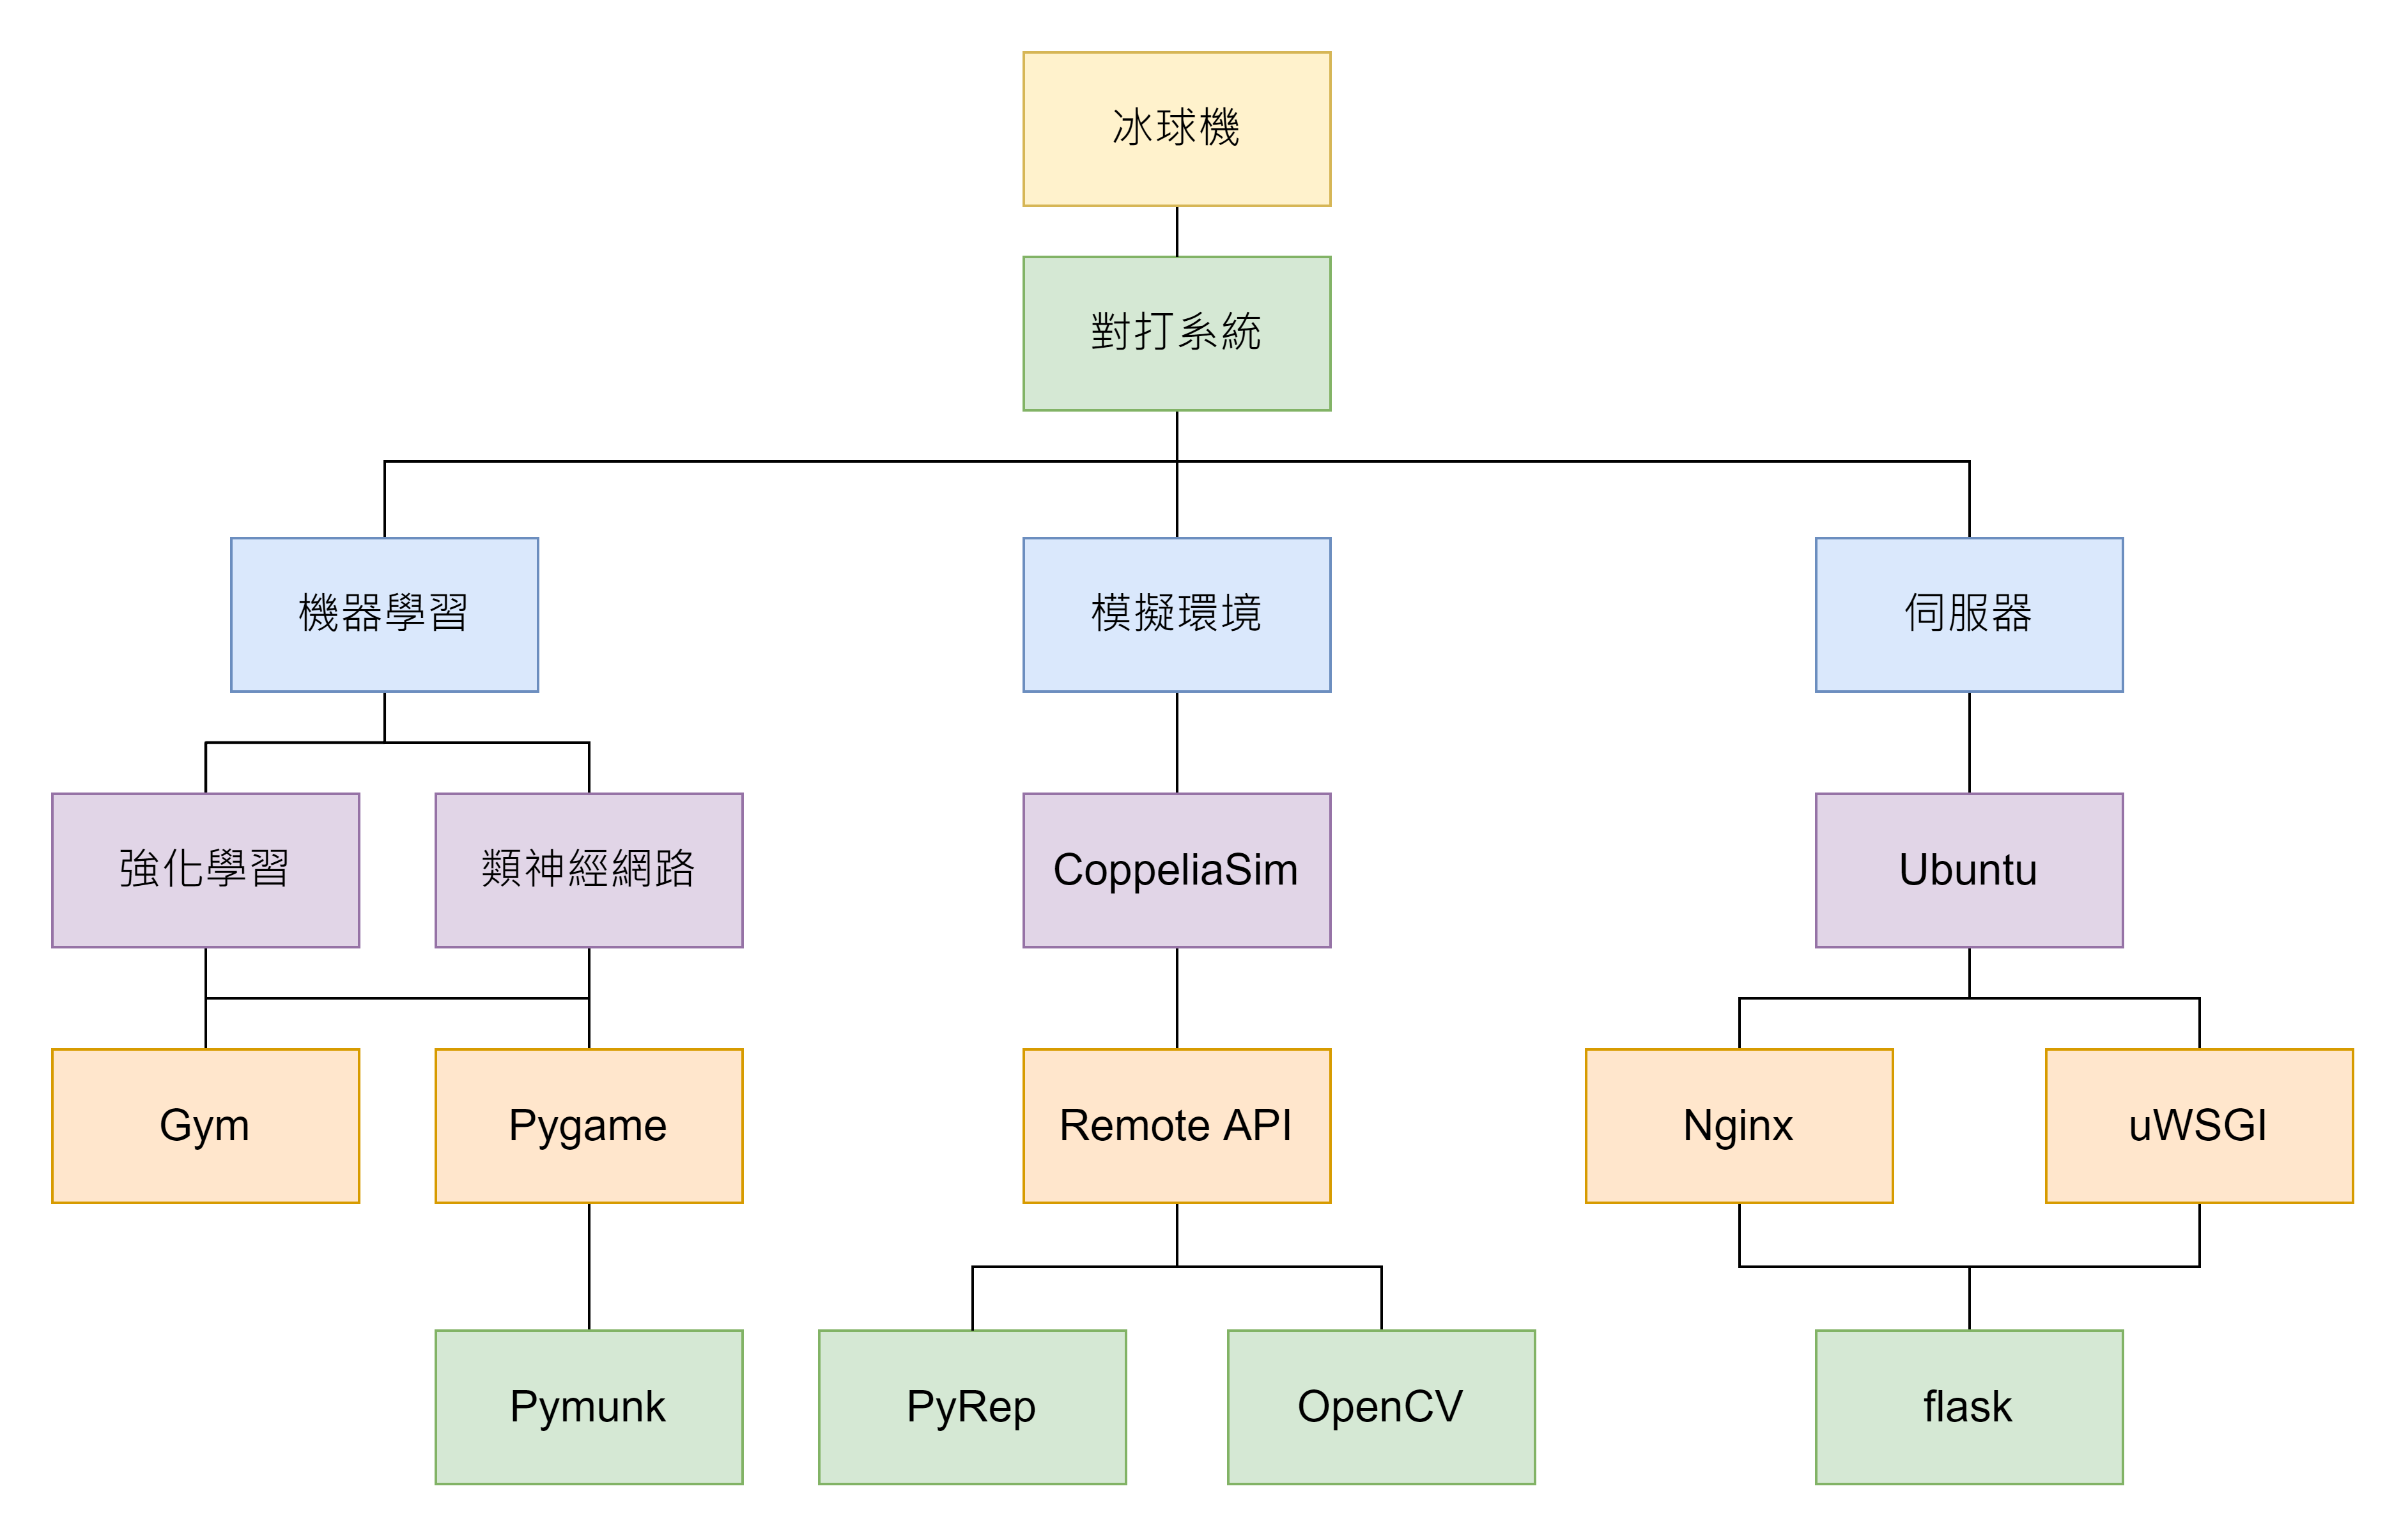
\includegraphics[width=15cm]{研究架構}
\caption{\Large 研究架構 }
\label{研究架構 }
\end{center}
\end{figure}
\section{未來展望}

\section{規則說明}
 Pong game 的遊戲規則簡單,透過擊錘將球打入對方球門即得一分,只要其中一方得21分就結束該局。擊錘只能沿單方向來回移動來進行防守和進攻。\\
遊戲規則如下:
\begin{enumerate}
\item 球打入敵方即得一分。
\item 擊錘只單一方向移動。
\item 最快贏得21分者獲勝,並結束該局遊戲。
\end{enumerate}

\renewcommand{\baselinestretch}{0.5} %設定行距